\documentclass[11pt]{article}
\usepackage[utf8]{inputenc}
\usepackage[T1]{fontenc}
\usepackage{fixltx2e}
\usepackage{graphicx}
\usepackage{grffile}
\usepackage{longtable}
\usepackage{wrapfig}
\usepackage{rotating}
\usepackage[normalem]{ulem}
\usepackage{amsmath}
\usepackage{textcomp}
\usepackage{amssymb}
\usepackage{capt-of}
\usepackage{hyperref}
\author{Pedro Cunial}
\date{\today}
\title{Descrição de Possiveis Projetos}
\hypersetup{
 pdfauthor={Pedro Cunial},
 pdftitle={B -- Detalhamento da proposta},
 pdfkeywords={},
 pdfsubject={},
 pdfcreator={Emacs 25.1.1 (Org mode 8.3.6)},
 pdflang={English}}
\begin{document}

\maketitle
\tableofcontents


\section{Cafeteira Despertador}
\subsection{Descrição da Ideia}
\label{sec:orgheadline1}
A ideia é construir um despertador que te acorde já com café pronto e quente
(recém feito).
\subsection{Diagrama de Blocos}
\label{sec:orgheadline2}
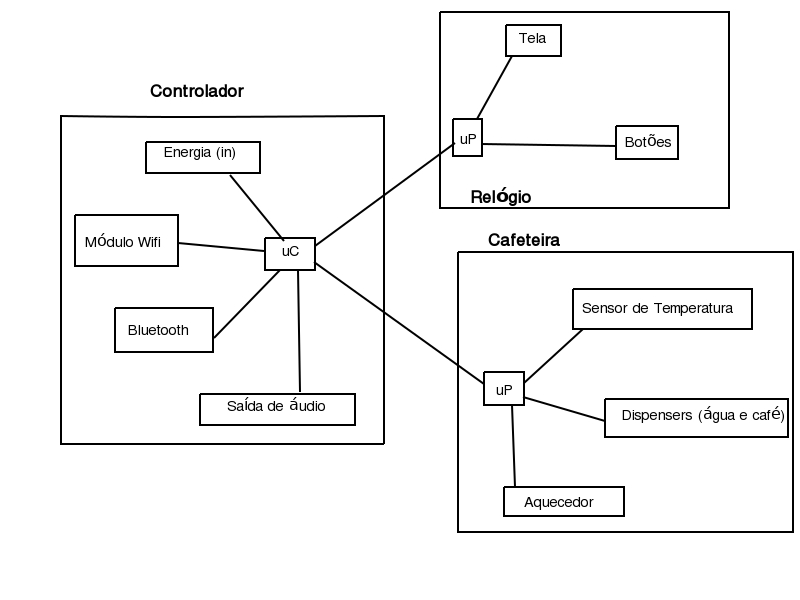
\includegraphics[width=\textwidth]{diagrama-cafeteira}
\subsection{Listagem de Tecnologias}
\label{sec:orgheadline3}
Para a realização do projeto, pretendo utilizar um micro-controlador principal
para gerenciar dois micro-processadores externos, um para o relógio e outro
para a cafeteira. A cafeteira deverá ter uma resistência para aquecer a água,
assim como um sensor de temperatura para garantir que a água de fato fora
aquecida e os dispensers de água e café.

O relógio precisa de um visor para as horas e um botão para desligar o
despertador, o controle de mudar as horas e definir o horário à despertar será
feito por wifi/bluetooth (ainda não tenho certeza qual das duas tecnologias
seria a melhor).
\subsection{Possíveis Gargalos}
\label{sec:orgheadline4}
Eu imagino que o principal gargalo do projeto será a parte da cafeteira,
principalmente a parte de automatizar todos os dispensers e temperatura da
água.

\section{Geladeira Individual}
\subsection{Descrição da Ideia}
\label{sec:orgheadline6}
A ideia é construir uma mini-geladeira para uma latinha de refrigerante, a
a temperatura esperada pode ser definida por uma aplicação (web ou mobile), de
forma que é possível resfriar algo na sua casa mesmo sem estar nela.
\subsection{Diagrama de Blocos}
\label{sec:orgheadline7}
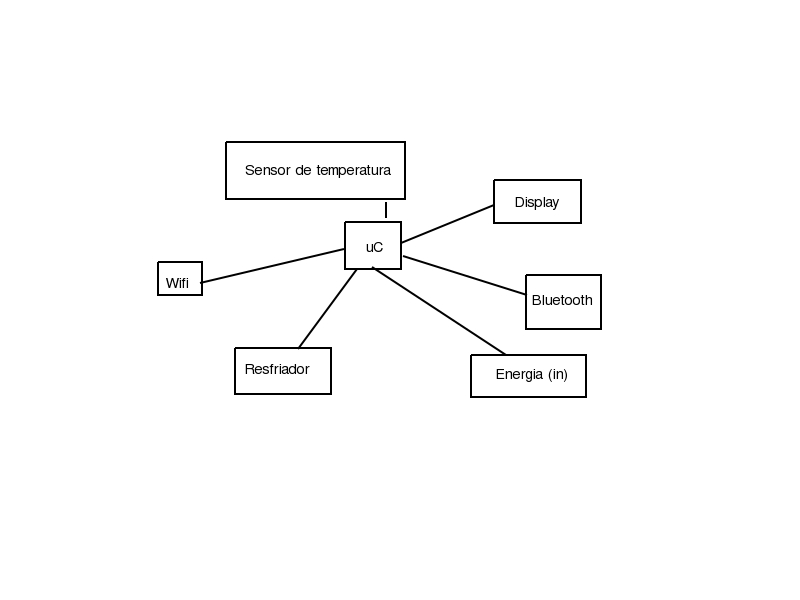
\includegraphics[width=\textwidth]{diagrama-refri}
\subsection{Listagem de Tecnologias}
\label{sec:orgheadline8}
Para a realização do projeto, pretendo utilizar um micro-controlador central, o
qual cuidará tanto de manter a temperatura na idea, quando em gerenciar o que
aparecerá no display e a troca de dados pelo wifi. Será necessário utilizar
alguma forma de resfriador para garantir que o ambiente realmente estará gelado
(o que ainda não tenho muita certeza de como fazer).
\subsection{Possíveis Gargalos}
\label{sec:orgheadline9}
Imagino que o principal gargalo vá ser a construção da ``mini-geladeira'' em si,
de forma que ela realmente seja ``hermeticamente segura'' e ainda assim seja
possível incluir um resfriador nela.
\end{document}